\subsection{Building the vocabulary} \label{implementation_vocab}

The first step of the implementation is building the vocabulary. Words that are not included in it will be discarded when computing the vector representations for the documents, venues and subjects. Therefore, it is a very important step. It should include all words  that are relevant for the task of \acrshort{si}, i.e. the words that describe the topics each document handles.

The vocabulary is directly extracted from the corpus (the titles and abstracts of the documents). Only words that appear in the documents can be present in the vocabulary. There are several design choices that should be considered. We use SpaCy's small trained pipeline (called ``en\_core\_web\_sm'') for tokenization. The lemmatization is performed by the WordNet lemmatizer of NLTK, using the \acrfull{pos} tags computed by Flair's sequence tagger. The reasoning behind these choices are discussed in the following sections.

\subsubsection{Tokenizer}

Tokens are the semantic units that \acrfull{nlp} pipelines build upon. They are usually words, but depending on the task at hand, one can tokenize strings in different ways. For example, \textit{aren't} can be kept as a token or divided into two tokens, \textit{are} and \textit{n't}. This kind of decisions are made by the tokenizer, an algorithm that divides a given text into tokens. Tokenizers are usually based on simple heuristics.

We use the tokenizer from spaCy\footnote{\url{https://spacy.io/usage/linguistic-features\#how-tokenizer-works}}. It tokenizes words (which are surrounded by white spaces) by iteratively looking for prefixes and suffixes until a match is found with a regular expression that defines how a token should look like. Another reason why we pick this tokenizer is because it is included in Flair \cite{akbik2019flair}, an \acrshort{nlp} framework which we use later on to compute the \acrshort{pos} tags of each token.

\subsubsection{N-grams} \label{vocab_ngrams}

In some cases, words pose different meanings when combined with others. For example, ``ice cream'' has a particular meaning, and it should therefore be present in the vocabulary as a phrase. The words ``ice'' and ``cream'' pose different meanings when used independently. Such phrases also occur in the scientific jargon. For instance, ``machine learning'' refers to a field of computer science, something that cannot be deduced from its name. Still, the name describes well the purpose of the field (teaching machines how to learn). This is usually the case with scientific terms: they aim to describe their application as clearly as possible.

We built a vocabulary with n-grams of up to length four, to see its size and constituent entries. After filtering out the ones that appeared in only one document and those that appear in more than 1,000 documents, we found out that the n-grams weren't as informative as we expected. Many of them were just common sequences of words, such as ``this is a problem''. We talk about this vocabulary in detail in the appendix. We decided against including n-grams because the increase in quality was low compared with the increase in computational cost. 

\subsubsection{Vocabulary normalization}

The purpose of normalizing a vocabulary is to reduce its size by grouping words with similar meanings together. We will now introduce two normalization techniques that we have included in our procedure: case folding and lemmatization.

\paragraph{Case folding} \mbox{}

The most straight-forward way of reducing the size of the vocabulary is case folding. For example, the word ``here'' may be capitalized because it is at the beginning of the sentence and would thus appear as another entry in the vocabulary. Writing all words in lower case eliminates this duplicity issue.

Case folding is not suitable for tasks where proper nouns should be identified. For example, the word ``frank'' has a different meaning than the name ``Frank''. This issue is not relevant for our task, as we are mainly interested in scientific words that have unique meanings. Therefore, we perform case folding on all words before adding them to the vocabulary.

\paragraph{Lemmatization} \mbox{}

Lemmatization consists of replacing words by their semantic roots. It makes the model more general by removing verb conjugations, plural cases and other variations of words that ultimately have the same meaning. This technique may also reduce the precision of the model. For instance, words with different meanings, such as ``bank`` and ``banking'', are reduced to the same lemma even if the meaning of the word ``bank'' is context-dependent. Such situations are a priori not dangerous for our task, as scientific words usually have concise meanings.

Stemming is a similar approach, in which prefixes and suffixes are removed. For example, the stem of the word ``house'' is ``hous'' and its lemma is ``house''. Lemmatization is more accurate because it takes into account the meaning of the word \cite{hapke2019natural}. A good example of this is ``better'', whose lemma is ``good'' while its stem is ``bet'', which has a completely different meaning. Because of this, lemmatizers are suitable for more applications, and ours is no exception.

We use the WordNet lemmatizer of the NLTK package in our pipeline. WordNet \cite{fellbaum2010wordnet} is a lexical database that is publicly available and offers lemmatization. NLTK provides an interface to this lemmatizer. The accuracy of the lemmatization improves when the \acrfull{pos} tag of the word that should be lemmatized is also provided. We do so using the fast universal \acrshort{pos} tagger from Flair \cite{akbik2019flair}, called ``upos-fast''. The model, which combines Flair's contextual word embeddings \cite{akbik2018contextual} with a LSTM-CRF model, is trained on the data set of the CoNLL's shared task of 2018 \cite{zeman2018conll}, which comprises words in 12 languages. The resulting tagger has an F1-score of 98.47\footnote{As seen here (accessed on 06.07.2021): \url{https://github.com/flairNLP/flair/blob/master/resources/docs/TUTORIAL_2_TAGGING.md}} on the Ontonotes data set, only behind its larger version, called ``upos''. The difference between them is too small (0.13) to account for the large difference in performance. Using the faster model speeds up the procedure by around 500 \%.

\subsubsection{Vocabulary filtering} \label{vocab_filtering}

Once the vocabulary has been created, we remove the entries that occur in only one document, as their meanings may be too specific to relate documents to one another. Entries that are either stop words\footnote{For this purpose, we use NLTK's list of English stop words, which comprises 179 words as of 07/07/2021.} or punctuation signs are also discarded. Symbols such as Greek letters are kept, as they refer to certain concepts in fields like Physics or Mathematics.

At first, we discarded entries that occur in more than 1,000 documents, which reduced the size of the vocabulary to 49,651 entries. However, this also resulted in 7,188 documents not having any words that were in the vocabulary, meaning that they could not be vectorized. Given that there are only 488 vocabulary entries that occur in more than 1,000 documents, we decided to keep them. This greatly improves the coverage: now only 85 documents cannot be represented.

\subsubsection{Resulting vocabulary} \label{vocab_results}

In our corpus, there are 125,575 distinct tokens. 75,436 of them appear in only one document and are discarded. Thus, the final vocabulary comprises 50,139 entries. With this vocabulary, only 85 documents cannot be represented, i.e. none of the words of their titles and abstracts appear on the vocabulary. Keep in mind that 51 of those documents didn't have any texts to begin with, as stated in section \ref{repo_analysis_data}.

In figure \ref{fig:bow_data}, the number of tokens of the documents that are included in the vocabulary is displayed. As mentioned before, 85 documents don't have any of their tokens in the vocabulary. 110 have just one. On the other end of the spectrum, 24,819 documents have nine or more tokens in the vocabulary. This accounts for 84 \% of all documents. Vocabulary entries appear on average on 27.1 documents. Figure \ref{fig:vocab_1grams} shows in how many documents each entry of the vocabulary occurs, grouped in bins. 46,776 entries (94 \%) appear in 100 documents or fewer. 15,250 entries (31 \%) appear in only two documents.

\begin{figure}
    \centering
    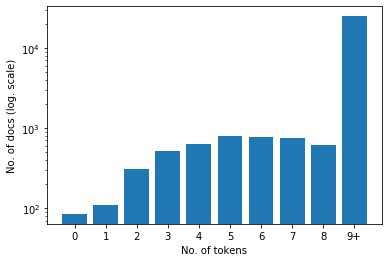
\includegraphics[width=.7\textwidth]{figures/unsupervised_approach/bow_data.png}
    \caption{Distribution of the documents depending on the number of their tokens that are included in the vocabulary.}
    \label{fig:bow_data}
\end{figure}

\begin{figure}
    \centering
    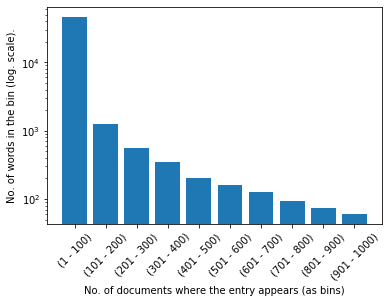
\includegraphics[width=.7\textwidth]{figures/vocab/vocab_1grams.png}
    \caption{Distribution of the vocabulary entries depending on the no. of documents they are included in.}
    \label{fig:vocab_1grams}
\end{figure}